% =====================================================================
% Tarea 2 - Machine Learning - Home Credit Default Risk
% Plantilla IEEE (IEEEtran, conference) — formato exigido en la pregunta
% de codigo fuente de hw02-2026-2.docx
% Estructura de secciones: hw02-2026-2.docx, "ESTRUCTURA DEL INFORME"
% =====================================================================
\documentclass[conference]{IEEEtran}
\IEEEoverridecommandlockouts

\usepackage{cite}
\usepackage{amsmath,amssymb,amsfonts}
\usepackage{graphicx}
\usepackage{booktabs}
\usepackage{textcomp}
\usepackage{xcolor}
\usepackage{cuted} % entorno "strip": contenido a una columna dentro de un
                    % documento a dos columnas (usado para la sección de
                    % Código Fuente, Courier 8pt de ancho completo)
\usepackage{listings}
\usepackage{caption}

% ---------------------------------------------------------------------
% Bloque de codigo fuente: Courier New 8pt, una sola columna, cada
% funcion/metodo "encuadrada" (frame=single). Requisito literal de
% hw02-2026-2.docx: "programa principal debe denominarse mainProcess".
% El bloque \begin{strip}...\end{strip} (provisto por IEEEtran) es lo que
% permite que el codigo rompa el layout de dos columnas y ocupe el ancho
% completo de la pagina, tal como exige el enunciado.
% ---------------------------------------------------------------------
\lstdefinestyle{codigoFuente}{
    basicstyle=\fontfamily{pcr}\selectfont\footnotesize, % Courier ~8pt
    frame=single,
    framerule=0.6pt,
    rulecolor=\color{black},
    breaklines=true,
    breakatwhitespace=false,
    tabsize=4,
    showstringspaces=false,
    columns=fullflexible,
    keepspaces=true,
    numbers=left,
    numberstyle=\tiny,
    xleftmargin=1.5em,
    captionpos=b,
}
\lstset{style=codigoFuente, language=Python}

\begin{document}

% =====================================================================
% TITULO, AUTOR Y FILIACION
% =====================================================================
\title{Análisis Exploratorio, Limpieza, Codificación, Balanceo y Ranking\\
de Atributos sobre el Dataset Home Credit Default Risk}

\author{
\IEEEauthorblockN{Mondragon Contreras, Sergio}
\IEEEauthorblockA{
Curso de Machine Learning \\
Tarea 2 -- 31 de julio de 2026
}
}

\maketitle

% =====================================================================
\begin{abstract}
% RESUMEN — completar al final, cuando el desarrollo este cerrado:
% objetivo, metodo, resultados numericos clave, conclusion principal.
Resumen pendiente de completar.
\end{abstract}

\begin{IEEEkeywords}
Home Credit Default Risk, EDA, calidad de datos, balanceo de clases,
selección de atributos, PCA
\end{IEEEkeywords}

% =====================================================================
\section{Introducción}

Este informe desarrolla la Tarea 2 del curso de Machine Learning: un
análisis exploratorio, de calidad, limpieza, codificación, balanceo y
selección de atributos sobre el dataset público de la competencia Kaggle
\emph{Home Credit Default Risk}. El desarrollo completo (código,
resultados intermedios y figuras) se produjo en un notebook Jupyter
(\texttt{notebooks/tarea2\_home\_credit.ipynb}) y se resume en este
documento siguiendo la estructura y el formato exigidos por el enunciado
de la tarea.

\textbf{Estado de este informe:} las secciones IV-A, IV-B y IV-C
(pasos 1 a 3 del procedimiento) están desarrolladas con resultados reales,
obtenidos ejecutando el notebook contra el archivo de datos completo. Las
secciones IV-D a IV-H (pasos 4 a 8) están en desarrollo activo y se
completan en una iteración posterior de este mismo documento.

% =====================================================================
\section{El Problema}

Se cuenta con datos reales de solicitudes de crédito de la entidad Home
Credit, incluyendo si cada solicitante terminó incumpliendo con su pago
(columna \texttt{TARGET}). El problema, en términos propios, consiste en
explorar a fondo ese conjunto de datos --- entender su estructura, medir
su calidad, corregir sus defectos, transformarlo a una forma que un
algoritmo de aprendizaje pueda consumir, y determinar qué atributos
concentran la mayor capacidad para anticipar si un cliente va a incumplir
--- como paso previo, necesario y no trivial, a la construcción de
cualquier modelo predictivo de riesgo crediticio. Le importa a Home
Credit porque su modelo de negocio depende de extender crédito
responsablemente a personas sin historial crediticio tradicional: un
modelo de riesgo deficiente termina rechazando a buenos pagadores o
aprobando a quienes no podrán pagar.

% =====================================================================
\section{Metodología de Trabajo}

El procedimiento sigue ocho pasos, en este orden, cada uno con su propio
ciclo de código, explicación y conclusión parcial, según lo exigido en la
sección PROCEDIMIENTO de \texttt{hw02-2026-2.docx}:

\begin{enumerate}
\item Descripción del problema y origen de los datos.
\item Descripción general del dataset (forma, tipos de dato, rangos).
\item Análisis de la variable \texttt{TARGET} (balance de clases).
\item Calidad de los datos (nulos, outliers, duplicados) y primer EDA.
\item Limpieza de datos y segundo EDA (post-limpieza).
\item Conversión de atributos categóricos a numéricos y tercer EDA.
\item Balanceo de clases.
\item Ranking de atributos por capacidad predictiva (técnicas \emph{Filter}),
      con histogramas por clase, dispersión y PCA.
\end{enumerate}

Los pasos 4 y 5 (Calidad y Limpieza) están explícitamente ponderados con
mayor peso en la evaluación de la tarea, por lo que reciben el mayor nivel
de detalle. El paso 8 depende de que el paso 7 (balanceo) ya se haya
completado.

% =====================================================================
\section{Desarrollo de la Solución}

\subsection{Descripción del problema}

El archivo \texttt{application\_train.csv} proviene de la competencia
pública de Kaggle \emph{Home Credit Default Risk} (2018). Home Credit es
una institución financiera no bancaria fundada en 1997 en la República
Checa, que opera en 14 países y se especializa en otorgar préstamos a
personas con historial crediticio limitado o inexistente. Al año 2018
(fecha de referencia de la competencia), el grupo reportaba más de 29
millones de clientes y más de 160 millones de préstamos otorgados, la
mayoría en Asia.

Home Credit publicó el dataset en Kaggle retando a la comunidad a mejorar
sus modelos de predicción de riesgo de incumplimiento (\emph{default}).
El objetivo declarado de la competencia era doble: que clientes capaces
de pagar no sean rechazados injustamente por falta de historial
crediticio tradicional, y que los préstamos que sí se otorguen vengan con
un capital, plazo y calendario de pagos que el cliente pueda sostener
realmente.

Cada fila de \texttt{application\_train.csv} es una solicitud de préstamo,
identificada por \texttt{SK\_ID\_CURR}, con datos estáticos del
solicitante al momento de la solicitud (demográficos, financieros, de
vivienda, y puntajes normalizados de fuentes externas) y la columna
\texttt{TARGET}, que vale 1 si el cliente tuvo un pago tardío
significativo en alguno de los primeros plazos del crédito, y 0 en
cualquier otro caso.

La métrica de evaluación de la competencia original era el área bajo la
curva ROC (ROC-AUC) entre la probabilidad predicha de \texttt{TARGET=1} y
el valor observado --- se menciona como contexto porque condiciona qué
significa ``buen modelo'' en este dominio: dado que el dataset está
desbalanceado (Sección~\ref{sec:target}), el \emph{accuracy} sería una
métrica engañosa.

\textbf{Nota de alcance:} el dataset completo de Kaggle incluye 10
archivos. Esta tarea, por instrucción explícita del enunciado, usa
\textbf{solo} \texttt{application\_train.csv}; los demás archivos se
mencionan aquí únicamente como contexto de origen, no se cargan en el
análisis.

\subsection{Descripción general del dataset}

El dataset tiene \textbf{307\,511 filas y 122 columnas}. La Tabla~\ref{tab:tipos}
resume la composición por tipo de dato.

\begin{table}[htbp]
\caption{Tipos de dato en \texttt{application\_train.csv}}
\label{tab:tipos}
\centering
\begin{tabular}{lc}
\toprule
Tipo & N.\ de columnas \\
\midrule
Numérico (\texttt{int64}/\texttt{float64}) & 106 \\
Categórico (\texttt{object}/\texttt{str})  & 16 \\
\bottomrule
\end{tabular}
\end{table}

Dentro de las 106 columnas numéricas hay una mezcla heterogénea:
identificadores (\texttt{SK\_ID\_CURR}), indicadores binarios 0/1
(\texttt{FLAG\_MOBIL}, \texttt{FLAG\_EMP\_PHONE}), conteos enteros
(\texttt{CNT\_CHILDREN}, \texttt{CNT\_FAM\_MEMBERS}), montos continuos
(\texttt{AMT\_INCOME\_TOTAL}, \texttt{AMT\_CREDIT}) y variables de tiempo
relativas expresadas en días negativos (\texttt{DAYS\_BIRTH},
\texttt{DAYS\_EMPLOYED}). Esta heterogeneidad importa: no se puede tratar
toda columna ``numérica'' con la misma estrategia de limpieza o escalado,
aunque \texttt{pandas} las tipifique igual.

Entre las 16 categóricas, la cardinalidad es muy dispar: la mayoría tiene
entre 2 y 8 categorías (p.\,ej.\ \texttt{NAME\_CONTRACT\_TYPE},
\texttt{CODE\_GENDER}), mientras que \texttt{ORGANIZATION\_TYPE} tiene 58
categorías distintas. Esto condiciona directamente la
Sección~\ref{sec:encoding}: las de baja cardinalidad son candidatas
naturales a codificación One-Hot sin explotar en dimensionalidad,
mientras que \texttt{ORGANIZATION\_TYPE} necesita una técnica como
Frequency o Binary Encoding.

\textbf{Influencia en las secciones posteriores.} 307\,511 filas es un
volumen amplio para entrenar un modelo de clasificación binaria robusto
--- en principio suficiente para que la validación cruzada y las técnicas
de balanceo (SMOTE, Sección~\ref{sec:balanceo}) tengan margen para
generar/seleccionar ejemplos sin quedarse sin datos. Sin embargo, el
volumen total \emph{no resuelve} el problema de desbalance de clases: el
tamaño de muestra grande ayuda a la estabilidad estadística general, pero
no sustituye a una estrategia explícita de balanceo.

\subsection{Análisis del Target}
\label{sec:target}

La Tabla~\ref{tab:target} y la Fig.~\ref{fig:target} resumen la
distribución de la variable objetivo.

\begin{table}[htbp]
\caption{Distribución de la variable \texttt{TARGET}}
\label{tab:target}
\centering
\begin{tabular}{clr}
\toprule
Clase & Descripción & \% del total \\
\midrule
0 & No incumple (repaga a tiempo)        & 91.93\,\% \\
1 & Incumple (pago tardío significativo) & 8.07\,\%  \\
\bottomrule
\end{tabular}
\end{table}

\begin{figure}[htbp]
\centering
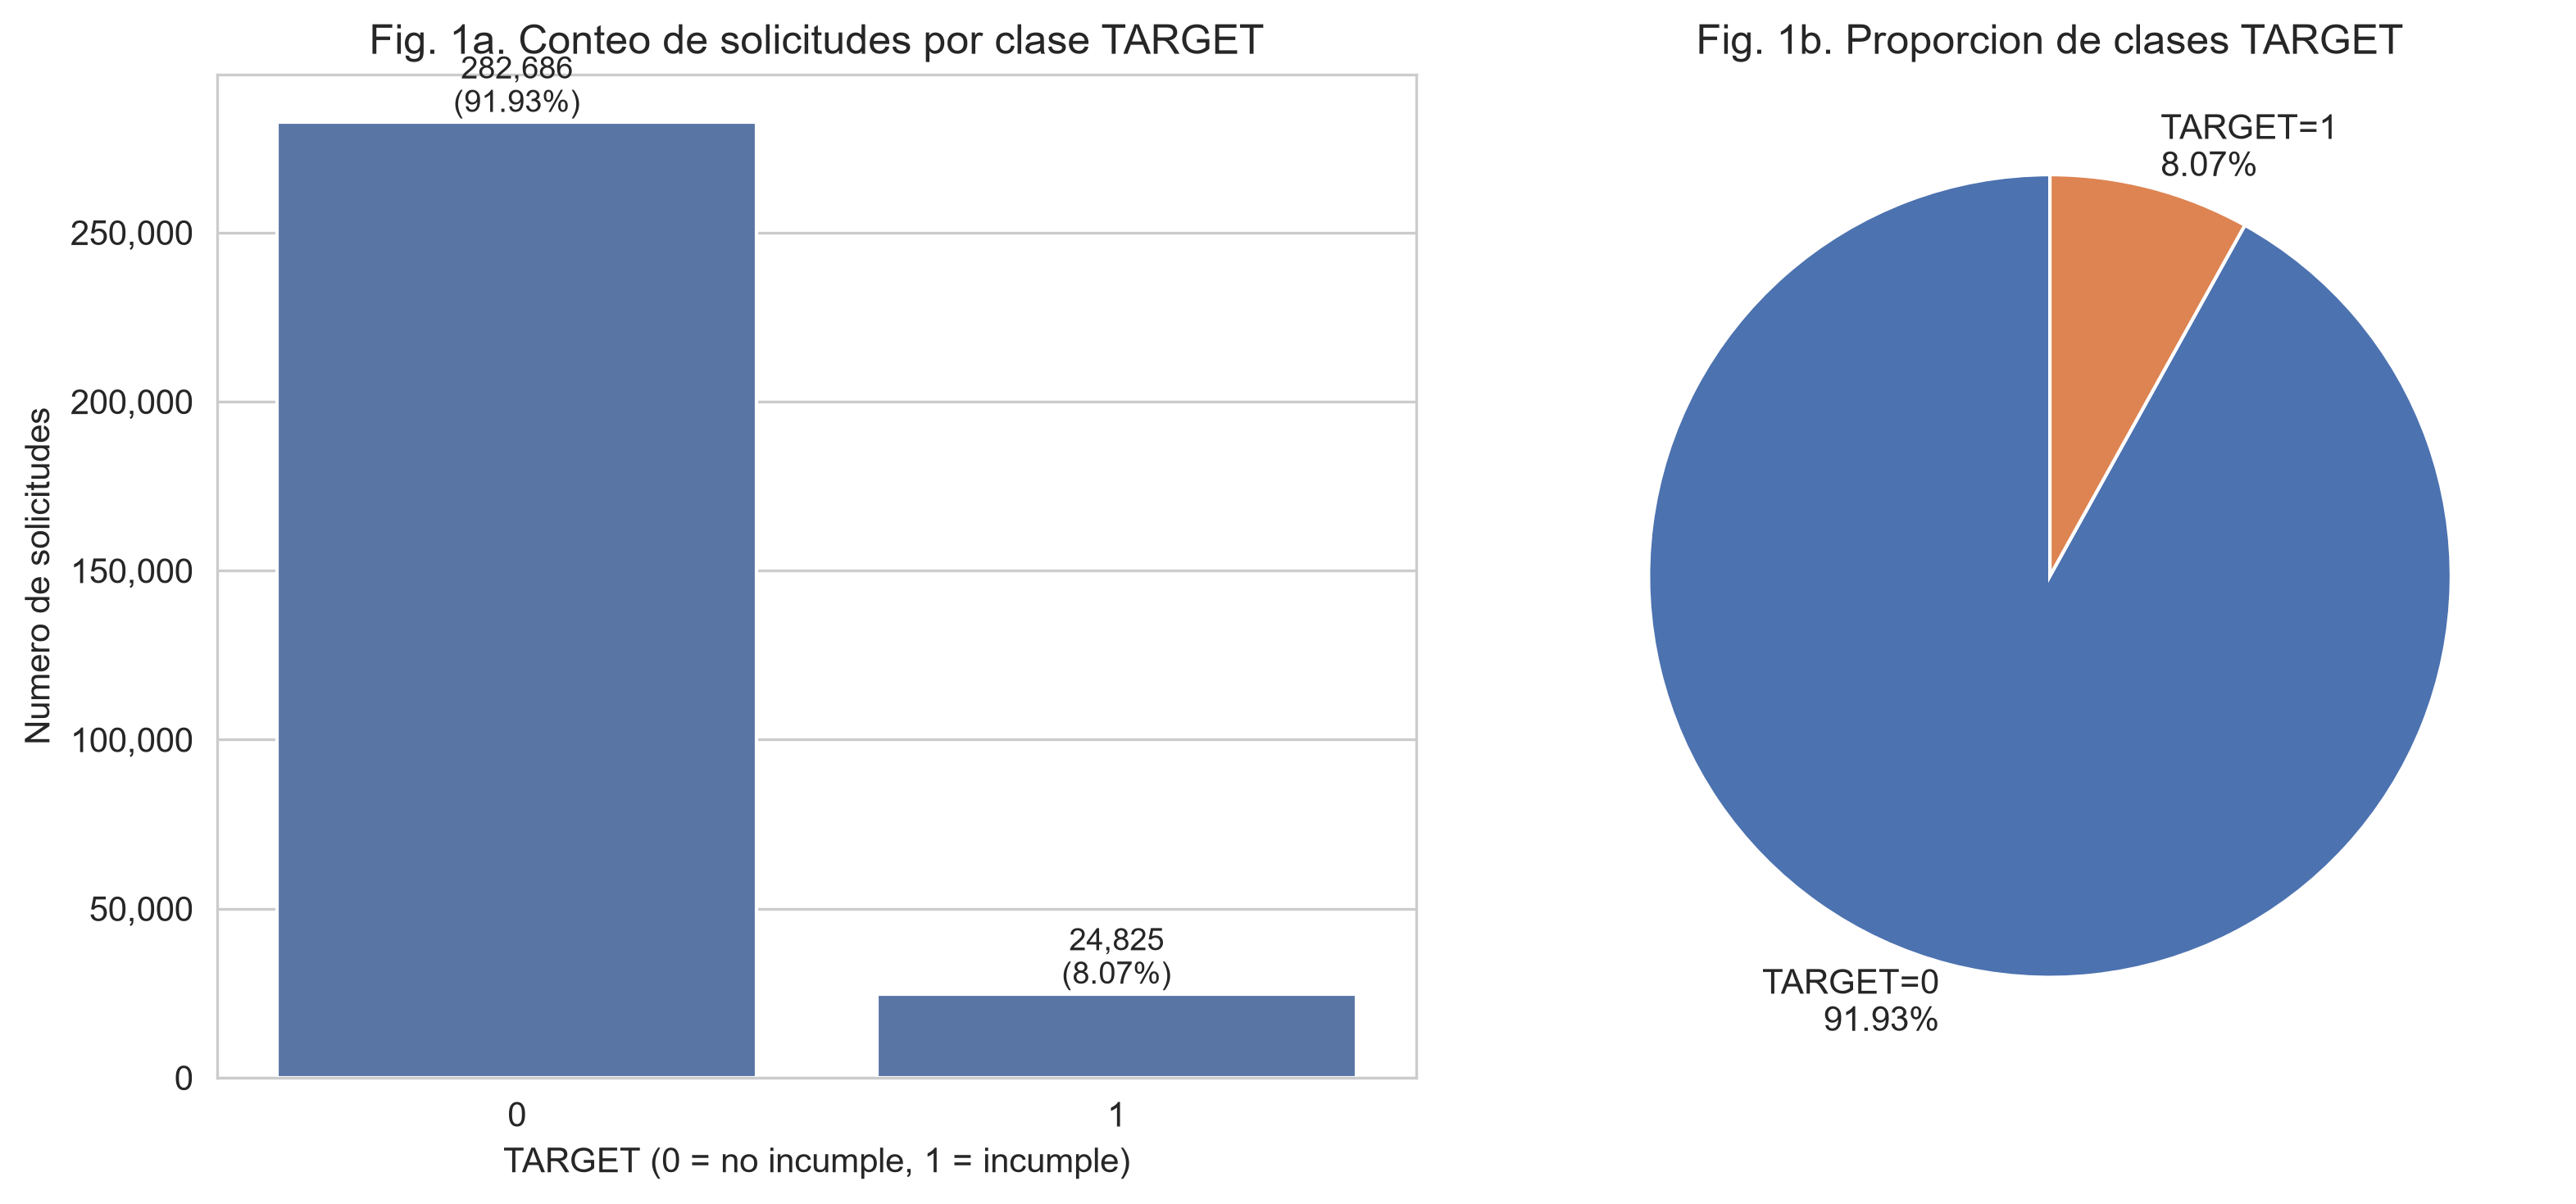
\includegraphics[width=\linewidth]{../output/figures/fig01_target_balance.png}
\caption{Conteo y proporción de solicitudes por clase \texttt{TARGET}.}
\label{fig:target}
\end{figure}

La clase \texttt{TARGET=0} representa 282\,686 solicitudes (91.93\,\%) y
la clase \texttt{TARGET=1} representa 24\,825 solicitudes (8.07\,\%) ---
una razón de aproximadamente 11.4 solicitudes que no incumplen por cada 1
que sí incumple.

\textbf{¿Están los datos balanceados?} No. El criterio operativo de este
informe es que una clase minoritaria por debajo del 10--20\,\% del total
ya constituye desbalance; aquí la clase minoritaria está en 8.07\,\%, por
debajo incluso del límite más estricto de ese rango. Es un desbalance
real y significativo, no marginal.

\textbf{Qué es el balanceo de datos y cómo afecta los resultados.} El
balanceo de datos es el conjunto de técnicas que corrigen, en los datos
de entrenamiento o en la función de pérdida del modelo, la disparidad en
la cantidad de ejemplos entre clases, de forma que el algoritmo no
termine optimizando casi exclusivamente para la clase mayoritaria. El
riesgo concreto de no balancear un dataset con esta proporción es que un
modelo puede alcanzar una exactitud engañosamente alta ($\sim$92\,\%) con
la estrategia trivial de predecir siempre \texttt{TARGET=0}. En términos
de métricas de clasificación, el desbalance típicamente hunde el
\emph{recall} y el F1-score de la clase minoritaria mientras la precisión
global se mantiene artificialmente alta --- exactamente el motivo por el
que la competencia original evalúa con ROC-AUC y no con \emph{accuracy}.

\textbf{Postura propia.} En un problema de riesgo crediticio como este,
el costo de los dos tipos de error no es simétrico: dejar pasar un
cliente que va a incumplir (falso negativo) le cuesta dinero real a Home
Credit, mientras que rechazar por error a un cliente que sí habría pagado
(falso positivo) es un costo de oportunidad, no una pérdida directa. Esto
sugiere que el balanceo no debería tratarse solo como un paso técnico
para ``limpiar'' el desbalance estadístico, sino como una decisión
alineada con esa asimetría de costos --- preferir una técnica que
privilegie el \emph{recall} de la clase \texttt{TARGET=1} sobre la
precisión general. Este criterio se retoma en la Sección~\ref{sec:balanceo}.

\subsection{Calidad de los Datos}
\textit{[Pendiente de desarrollo --- paso 4 del procedimiento. Se
documentarán aquí: \% de nulos por columna, filas con nulos,
outliers/valores inconsistentes, duplicados y columnas de una sola
categoría, junto con el primer EDA completo (Anexo 1 de
\texttt{hw02-2026-2.docx}).]}

\subsection{Limpieza de Datos}
\textit{[Pendiente de desarrollo --- paso 5. Incluirá el tratamiento del
valor centinela \texttt{365243} en \texttt{DAYS\_EMPLOYED} y el criterio
de retención de \texttt{EXT\_SOURCE\_1} pese a su 56\,\% de nulos.]}

\subsection{Conversión de Atributos Categóricos en Numéricos}
\label{sec:encoding}
\textit{[Pendiente de desarrollo --- paso 6. Aplicará las técnicas del
Anexo 2 (Label, One-Hot, Ordinal, Frequency, Binary) según el tipo de
cada una de las 16 columnas categóricas.]}

\subsection{Balanceo de Datos}
\label{sec:balanceo}
\textit{[Pendiente de desarrollo --- paso 7. Técnica candidata: SMOTE o
\texttt{class\_weight='balanced'} (ver justificación preliminar en
Sección~\ref{sec:target} y Anexo 3 de \texttt{hw02-2026-2.docx}).]}

\subsection{Ranking de Atributos según su Capacidad Predictiva}
\textit{[Pendiente de desarrollo --- paso 8, condicionado a que el paso 7
esté completo. Usará técnicas \emph{Filter} (\texttt{f\_classif},
\texttt{mutual\_info\_classif}, \texttt{chi2}, correlación), con
histogramas por clase, dispersión de atributos seleccionados, y PCA sobre
atributos originales vs.\ seleccionados.]}

% =====================================================================
\section{Resultados}
\textit{[Pendiente --- se completa cuando cierren los 8 pasos del
desarrollo.]}

% =====================================================================
\section{Conclusiones}
\textit{[Pendiente --- con indicadores numéricos, no opiniones. Hasta
ahora, verificado: el dataset tiene 307\,511$\times$122 (Sección IV-B) y
un desbalance de clases de 11.4:1 que requiere corrección explícita antes
de modelar (Sección IV-C).]}

% =====================================================================
\section{Recomendaciones}
\textit{[Pendiente --- mínimo 3, con análisis de viabilidad, se redactan
al cierre del desarrollo.]}

% =====================================================================
\section{Código Fuente}
% Requisito literal: Courier New 8pt, una sola columna (\begin{strip}),
% cada funcion/metodo encuadrado, programa principal llamado mainProcess.
% Codigo de produccion identico al de notebooks/tarea2_home_credit.ipynb
% (clase HomeCreditAnalysis + mainProcess), ya ejecutado y verificado
% contra el dataset completo (ver Secciones IV-B y IV-C). Diseño OOP:
% una clase orquestadora, un metodo por paso del procedimiento -- el
% estado (self.df y resultados intermedios) se comparte entre metodos
% sin pasarlo por parametro.
\begin{strip}

\begin{lstlisting}[caption={Clase \texttt{HomeCreditAnalysis} -- un método por paso del procedimiento}, label={lst:analysis}]
class HomeCreditAnalysis:
    """Orquesta el analisis completo de application_train.csv
    (Tarea 2). Cada metodo publico implementa un paso del
    procedimiento exigido por hw02-2026-2.docx. El estado se
    guarda como atributos de instancia para que los pasos
    posteriores lo reutilicen sin recibirlo/devolverlo por
    parametro."""

    def __init__(self, data_path="../data/application_train.csv",
                 figures_dir="../output/figures",
                 tables_dir="../output/tables", dpi=300):
        self.data_path = data_path
        self.figures_dir = figures_dir
        self.tables_dir = tables_dir
        self.dpi = dpi
        self.df = None
        self.resumen_tipos = None
        self.cardinalidad = None
        self.numeric_summary = None
        self.resumen_target = None

    def cargar_datos(self):
        """Paso 1-2 (carga): unico archivo en el alcance."""
        self.df = pd.read_csv(self.data_path)
        print(f"application_train.csv -> filas: "
              f"{self.df.shape[0]:,}  columnas: {self.df.shape[1]}")
        return self.df

    def describir_dataset(self):
        """Paso 2: tipos de dato, cardinalidad, Tabla I."""
        df = self.df
        # pandas 3.x reporta columnas de texto como dtype "str"
        # (antes "object") -- se cuentan ambas etiquetas.
        dtype_counts = df.dtypes.astype(str).value_counts()
        n_numericas = int(dtype_counts.get("int64", 0)
                           + dtype_counts.get("float64", 0))
        n_categoricas = int(dtype_counts.get("object", 0)
                             + dtype_counts.get("str", 0))

        cat_cols = df.select_dtypes(include="object").columns.tolist()
        self.cardinalidad = (df[cat_cols].nunique()
                              .sort_values(ascending=False))

        self.numeric_summary = (df.select_dtypes(include=[np.number])
                                 .describe().T)
        self.numeric_summary["rango"] = (self.numeric_summary["max"]
                                          - self.numeric_summary["min"])

        self.resumen_tipos = pd.DataFrame({
            "tipo": ["numerico (int64/float64)",
                     "categorico (object/str)"],
            "n_columnas": [n_numericas, n_categoricas],
        })
        self.resumen_tipos.to_csv(
            f"{self.tables_dir}/tabla01_tipos_de_dato.csv", index=False)
        return self.resumen_tipos, self.cardinalidad

    def analizar_target(self):
        """Paso 3: balance de clases, Tabla II y Fig. 1."""
        df = self.df
        target_counts = df["TARGET"].value_counts().sort_index()
        target_pct = (target_counts / target_counts.sum()
                      * 100).round(2)
        self.resumen_target = pd.DataFrame({
            "clase": target_counts.index,
            "conteo": target_counts.values,
            "porcentaje": target_pct.values,
        })
        self.resumen_target.to_csv(
            f"{self.tables_dir}/tabla02_balance_target.csv",
            index=False)

        fig, axes = plt.subplots(1, 2, figsize=(11, 5))
        sns.barplot(x=self.resumen_target["clase"].astype(str),
                    y=self.resumen_target["conteo"], ax=axes[0],
                    color="#4C72B0")
        axes[0].set_title(
            "Fig. 1a. Conteo de solicitudes por clase TARGET")

        etiquetas = [f"TARGET={c}\n{p}%" for c, p in
                     zip(self.resumen_target["clase"],
                         self.resumen_target["porcentaje"])]
        axes[1].pie(self.resumen_target["conteo"], labels=etiquetas,
                    colors=["#4C72B0", "#DD8452"], startangle=90)
        axes[1].set_title("Fig. 1b. Proporcion de clases TARGET")

        plt.tight_layout()
        plt.savefig(f"{self.figures_dir}/fig01_target_balance.png",
                    dpi=self.dpi, bbox_inches="tight")
        plt.close(fig)
        return self.resumen_target

    # TODO paso 4: calidad_de_los_datos(self)
    # TODO paso 5: limpiar_datos(self)
    # TODO paso 6: convertir_categoricas(self)
    # TODO paso 7: balancear_clases(self)
    # TODO paso 8: ranking_atributos(self)
\end{lstlisting}

\begin{lstlisting}[caption={mainProcess -- orquestador principal del análisis}, label={lst:mainprocess}]
def mainProcess():
    """
    Punto de entrada unico del analisis (Tarea 2).
    Pasos 1-3 implementados y verificados contra el dataset
    completo (307,511 x 122). Pasos 4-8 (calidad, limpieza,
    encoding, balanceo, ranking+PCA) en desarrollo -- ver
    hw02-2026-2.docx, seccion PROCEDIMIENTO.
    """
    analysis = HomeCreditAnalysis()
    analysis.cargar_datos()
    analysis.describir_dataset()
    analysis.analizar_target()

    # TODO paso 4: analysis.calidad_de_los_datos()
    # TODO paso 5: analysis.limpiar_datos()
    # TODO paso 6: analysis.convertir_categoricas()
    # TODO paso 7: analysis.balancear_clases()
    # TODO paso 8: analysis.ranking_atributos()

    return analysis


if __name__ == "__main__":
    mainProcess()
\end{lstlisting}

\end{strip}

% =====================================================================
\bibliographystyle{IEEEtran}
\begin{thebibliography}{2}

\bibitem{kuhn2019}
M.~Kuhn and K.~Johnson, \emph{Feature Engineering and Selection: A
Practical Approach for Predictive Models}. Boca Raton, FL, USA: Chapman
\& Hall/CRC Press, 2019.

\bibitem{he2013}
H.~He and Y.~Ma, \emph{Imbalanced Learning: Foundations, Algorithms and
Applications}. Hoboken, NJ, USA: Wiley-IEEE Press, 2013.

\end{thebibliography}

\end{document}
